\chapter{Numerical Ordinary Differential Equations}\label{ch:odes}

In this chapter we will solve first order ordinary differential equations of the form
\[ y'(t) = f(t,y(t)) \]
with initial condition $y(t_0)=y_0$ for $t\ge t_0$.  These are known as ``ordinary''
differenatial equations since they contain only ``ordinary'' derivatives; not partial
derivatives.  Given that we are solving the problem with given intial information these
are also called intial value problems.  

\section{Euler, Runge-Kutta, and Friends}
The notion of approximating solutions to differential equations is simple: make a discrete
approximation to the derivative and step forward through time as a difference equation.
The fun part is making the approximation to the derivative(s).  There are many methods for
approximating derivatives, and that is exactly where we'll start.

\begin{technique}[Euler's Method]
    You're probably already familiar with Euler's method for approximating the solution to
    a differential equation. We want to approximate a solution to $y'(t) = f(t,y(t))$.
    Recall from Problem \ref{prob:num_diff_first_order} that 
    \[ y'(t) = \frac{y(t+h) - y(t)}{h} + \mathcal{O}(h) \]
    so the differential equation $y'(t) = f(t,y(t))$ becomes
    \[ \frac{y(t+h) - y(t)}{h} \approx f(t,y(t)). \]
    Rewriting as a difference equation, letting $y_{n+1} = y(t_n+h)$ and $y_n = y(t_n)$,
    we get
    \begin{flalign}
        y_{n+1} = y_n + h f(t_n , y_n)
        \label{eqn:Eulers_method}
    \end{flalign}
%     \begin{enumerate}
%         \item Recall that a taylor series for a continuously differentiable function
%             $f(x)$ centered at $x=a$ is
%             \[ f(x) = f(c) + \frac{f'(a)}{1!}(x-a) + \frac{f''(a)}{2!}(x-a)^2 +
%                 \frac{f^{(3)}(a)}{3!}(x-a)^3 + \frac{f^{(4)}(a)}{4!}(x-a)^4 + \cdots \]
%         \item Write a Taylor series for $y(t)$ by replacing $f$ with $y$, $x$ with $t+h$
%             and $a$ with $t$
%             \[ y(t+h) = \dots\]
% %             \teacher{
% %                 \[ y(t+h) = y(t) + y'(t)h + \frac{y''(t)}{2!} h^2 + \cdots \]
% %             }
%         \item Since we know that $y'(t) = f(t,y(t))$ we can rewrite the Taylor series as
%             \[ y(t+h) = \dots \]
% %             \teacher{
% %                 \[ y(t+h) = y(t) + hf(t,y(t)) + \frac{y''(t)}{2!} h^2 + \cdots \]
% %             }
%         \item Now we can look at this as a difference equation that is ready made for
%             numerical implementation with a loop:
%             \[ y_{n+1} = y_n + h f(t_n,y_n) + \mathcal{O}(h^2)\]
%         \item The {\it approximation error} for Euler's method is actually not second
%             order as the previous equation would suggest.  Instead, if we rearrange to
%             write Euler's formula as an approximation of the derivative we get
%             \[ \frac{y_{n+1}-y_n}{h} = f(t_n,y_n) + \mathcal{O}(h). \]
%             What does this formula tell you about the accuracy of Euler's method?
%     \end{enumerate}
\end{technique}

A way to think about Euler's method is that at a given point, the slope is approximated by
the value of the right-hand side of the differential equation and then we step forward $h$
units in time following that slope.  Figure \ref{fig:Euler} shows a depiction of the idea.
Notice in the figure that in regions of high curvature Euler's method will overshoot the
exact solution to the differential equation.  However, taking $h \to 0$ theoretically
gives the exact solution at the tradeoff of needing infinite computational resources.

\begin{figure}[ht!]
    \begin{center}
        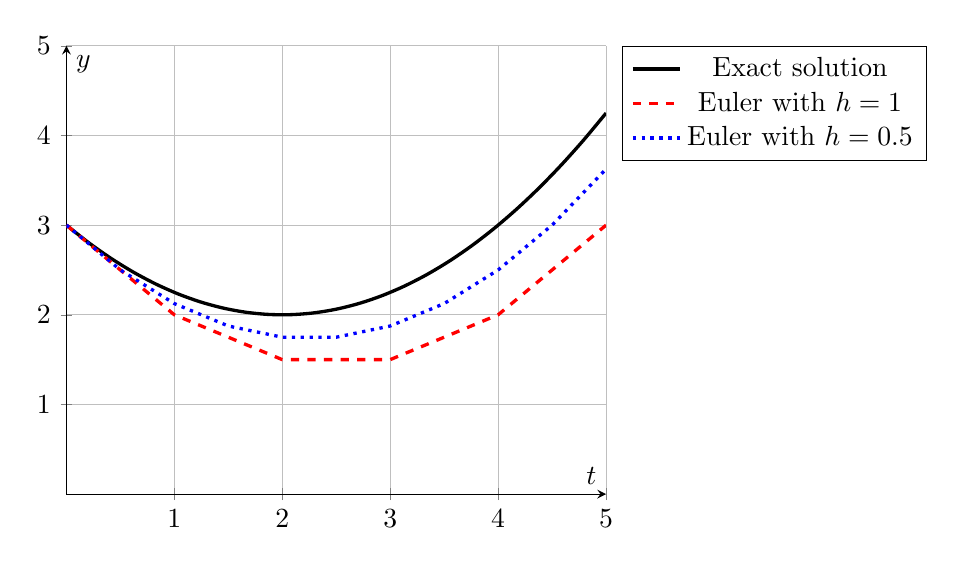
\begin{tikzpicture}
            \begin{axis}[axis lines=center, grid, xmin=0, xmax=5, ymin=0, ymax=5,
                domain=0:5, xlabel={$t$}, ylabel={$y$}, legend pos=outer north east]
                \addplot[very thick, smooth, black] {0.25*(x-2)^2+2};
                \addlegendentry{Exact solution};
                \addplot[red, dashed, very thick]
                coordinates{(0,3)(1,2)(2,1.5)(3,1.5)(4,2)(5,3)};
                \addlegendentry{Euler with $h=1$};
                \addplot[blue, dotted, very thick]
                coordinates{(0,3)(0.5,2.5)(1,2.125)(1.5,1.875)(2,1.75)(2.5,1.75)(3,1.875)(3.5,2.125)(4,2.5)(4.5,3)(5,3.625)};
                \addlegendentry{Euler with $h=0.5$};
            \end{axis}
        \end{tikzpicture}
    \end{center}
    \caption{A depiction of Euler's method with step size $h=1$ (red) and $h=0.5$ (blue).}
    \label{fig:Euler}
\end{figure}


\begin{problem}
    Write code to implement Euler's method for initial value problems.  Your MATLAB
    function should accept as input: $f(t,y)$, \mcode{tmin}, \mcode{tmax}, the number of
    grid points (the value of $h = \Delta t$ should be calculated within your code), and
    an intial condition.  The output should be vectors for $t$ and $y$.\\
    \mcode{function [t,y] = MyEuler1D(f,tmin,tmax,num_pts,IC)} \\
    Test your code on a first order differential equation where you know the answer and
    then test your code on the differential equation
    \[ y' = -\frac{1}{3}y+\sin(t) \quad \text{where} \quad y(0) = 1. \]
\end{problem}

\begin{problem}\label{prob:2dPredPrey}
    Write code that implements a 2D version of Euler's method that will solve a system of
    two differential equations in two dependent variables.  Test your code on the
    following problem by showing a time evolution plot (time on $x$ and populations on
    $y$) as well as a phase plot ($x$ on the $x$ and $y$ on the $y$ with time understood
    implicitly):\\
    {\bf The Lotka-Volterra Predator-Prey Model:}\\
    Let $x(t)$ denote the number of rabbits (prey) and $y(t)$ denote the number of foxes
    (prey) at time $t$.  The relationship between the species can be modeled by the
    classic 1920's Lotka-Volterra Model:
    \[ \left\{ \begin{array}{ll} x' &= \alpha x - \beta xy \\ y' &= -\delta y + \gamma xy
        \end{array} \right. \]
    where $\alpha, \beta, \gamma,$ and $\delta$ are positive constants.  For this
    problems take $\alpha \approx 1$, $\beta \approx 0.05$, $\gamma \approx 0.01$, and
    $\delta \approx 1$.  Be sure to explain the meaning of each of the parameters and each
    of the components of the model.
\end{problem}

\begin{technique}[The Midpoint Method]
    Now we begin the journey of creating better solvers than Euler's method.  The midpoint method
    is defined by first taking a half step with Euler's method to approximate a solution
    at time $t_{n+1/2} \equiv (t_n + t_{n+1})/2$ and then taking a full step using the
    value of $f$ at $t_{n+1/2}$ and the approximate $y_{n+1/2}$.
    \begin{flalign*}
        y_{n+1/2} &= y_n + \frac{h}{2} f(t_n, y_n) \\
        y_{n+1} &= y_n + h f(t_{n+1/2}, y_{n+1/2})
    \end{flalign*}
    Note: Indexing by $1/2$ in a computer is nonsense.  Instead, we implement the midpoint
    method with:
    \begin{flalign*}
        y_{temp} &= y_n + \frac{h}{2} f(t_n, y_n) \\
        y_{n+1} &= y_n + h f\left( \frac{t_n+t_{n+1}}{2}, y_{temp}\right)
    \end{flalign*}

\end{technique}

\begin{problem}
    Write MATLAB code to implement the midpoint method\\
    \mcode{function [t,y]=MyMidpointMethod(f,tmin,tmax,num_pts,IC)} \\
\end{problem}

\begin{problem}
    Test your midpoint method code against your Euler1D code on the same single variable
    ODE as before.  You will likely see very little difference on a very small step size
    (equivalently, a large number of points), but for a smaller number of points there
    will be a remarkable difference.  
\end{problem}


\begin{problem}
    {\bf The Runge-Kutta Method:}\\
    Another method for approximating the solution to a first order initial value problem
    is to take several approximations and average them in a smart way.  The Runge-Kutta 4
    method is one (of many) such methods.  In this method, each $k_j$ is an approximation
    of the slope and we combine them in as a weighted average in the end.
    \begin{flalign*}
        k_1 &= f(t_n, y_n) \\
        k_2 &= f(t_n + \frac{h}{2} , y_n + \frac{h}{2} k_1) \\
        k_3 &= f(t_n + \frac{h}{2} , y_n + \frac{h}{2} k_2) \\
        k_4 &= f(t_n + h , y_n + h k_3) \\
        y_{n+1} &= y_n + \frac{h}{6} \left( k_1 + 2 k_2 + 2 k_3 + k_4 \right)
    \end{flalign*}

    Write a MATLAB function that implements the Runge-Kutta 4 method in one dimension.\\
    \mcode{function [t,y]=MyRk4(f,tmin,tmax,num\_pts,IC)} \\
    Test the problem on a known differential equation.
\end{problem}


\begin{problem}
    Modify your Runge-Kutta 4 code to work for two dependent variables.  I'll get you
    started:\\We want to solve
    \[ \left\{ \begin{array}{ll} x' &= f(t,x,y) \\ y' &= g(t,x,y) \end{array} \right. \]
    and to do so we extend the Runge Kutta method as
    \begin{flalign*}
        k_1 &= f(t_n,x_n, y_n) \\
        q_1 &= g(t_n,x_n, y_n) \\
        k_2 &= f(t_n + \frac{h}{2} ,x_n+\frac{h}{2} k_1, y_n + \frac{h}{2} q_1) \\
        q_2 &= g(t_n + \frac{h}{2} ,x_n+\frac{h}{2} k_1, y_n + \frac{h}{2} q_1) \\
        k_3 &= \dots \\
        q_3 &= \dots \\
        k_4 &= \dots \\
        q_4 &= \dots \\
        x_{n+1} &= x_n + \frac{h}{6} \left( k_1 + 2 k_2 + 2 k_3 + k_4 \right)\\
        y_{n+1} &= y_n + \frac{h}{6} \left( q_1 + 2 q_2 + 2 q_3 + q_4 \right)
    \end{flalign*}
    
    Test your code on
    the predator prey model in problem \ref{prob:2dPredPrey}.
\end{problem}


\begin{problem}
    Solving systems of ordinary differential equations would become challenging if we were
    to continue coding in the same way as in the previous problem. Write a MATLAB function
    that accepts any number of right-hand sides from a system of differential equations
    and then leverages the fact that MATLAB works very well with vectors to create Euler
    and Runge-Kutta solutions to these systems. Devise several systems to test your code
    (including 1D and 2D).
\end{problem}


\section{Implicit Methods and Shooting Methods}
\begin{problem}
    The major trouble with the RK (and midpoint) methods is that they take many more
    function evaluations than Euler's method.  We can improve upon Euler's method in the
    following way:\\
    We want to solve $y' = f(t,y)$ so:
    \begin{enumerate}
        \item Approximate the derivative by looking forward in time(!)
            \[ \frac{y_{n+1} - y_n}{h} \approx f(t_{n+1} , y_{n+1}) \]
        \item Rearrange to get the difference equation
            \[ y_{n+1} = y_n + h f(t_{n+1},y_{n+1}). \]
        \item Notice that we \underline{will} have $t_{n+1}$ but we \underline{do not
            have} $y_{n+1}$.  The major trouble is that $y_{n+1}$ shows up on both sides
            of the equation.  Can you think of a way to solve for it? \dots you have code
            that does this step!!!
        \item This method is called the {\bf backward Euler} method and is known as an
            {\bf implicit method} since you need to solve a nonlinear equation at each
            step.  The advantage (usually) is that you can take far fewer steps with
            reasonably little loss of accuracy.
    \end{enumerate}
\end{problem}

\begin{problem}
    Write MATLAB code to implement the backward Euler's method for a 1D initial value
    problem. \\
    \mcode{function [t,y] = MyBackwardEuler(f, tmin, tmax, num_pts, IC)}
\end{problem}


\begin{problem}
    Write a MATLAB script that outputs a log-log plot with the step size on the horizontal
    axis and the error in the numerical method on the vertical axis.  Plot the errors for
    Euler, Midpoint, Runge Kutta, and Backward Euler measured against a differential
    equation with a known analytic solution.  Use this plot to conjecture the convergence
    rates of the four methods.
\end{problem}

\begin{problem}
    In this model there are two characters, Romeo and Juliet, whose affection is
    quantified on the scale from $-5$ to $5$ described below:
    \begin{center}
        \begin{tabular}{|c|c|}
            \hline
            $-5$ & Hysterical Hatred \\
            $-2.5$ & Disgust \\
            $0$ & Indifference \\
            $2.5$ & Sweet Affection \\
            $5$ & Ecstatic Love\\
            \hline
        \end{tabular}
    \end{center}
    The characters struggle with frustrated love due to the lack of reciprocity of their
    feelings.  Mathematically,
    \begin{itemize}
        \item Romeo: ``My feelinfs for Juliet decrease in proportion to her love for me.''
        \item Juliet: ``My love for Romeo grows in proportion to his love for me.''
        \item Juliet's emotional swings lead to many sleepless nights, which consequently
            dampens her emotions.
    \end{itemize}
    This give rise to
    \[ \left\{ \begin{array}{ll} \frac{dx}{dt} &= -\alpha y \\ \frac{dy}{dt} &= \beta x -
            \gamma y^2 \end{array} \right. \]
    where $x(t)$ is Romeo's love for Juliet and $y(t)$ is Juliet's love for Romeo at time
    $t$.

    Your tasks:
    \begin{enumerate}
        \item First implement this 2D system with $x(0) = 2$, $y(0)=0$, $\alpha=0.2$,
            $\beta=0.8$, and $\gamma=0.1$ for $t \in [0,60]$.  What is the fate of this
            pair's love under these assumptions?
        \item Write MATLAB code that approximates the parameter $\gamma$ that will result
            in Juliet having a feeling of indifference at $t=30$.  Your code should not
            need human supervision: you should be able to tell it that you're looking for
            {\it indifference} at $t=30$ and turn it loose to find an approximation for
            $\gamma$.  Assume throughout this problem that $\alpha=0.2$, $\beta=0.8$,
            $x(0)=2$, and $y(0)=0$. Write a description for how your code works in your
            homework document and also submit your MATLAB file (along with any support
            files) demonstrating how it works.
            \\
            Hint: One way to do this problem is very similar to a bisection method for
            root finding. 
            \begin{itemize}
                \item Shoot two solutions with two different parameters.
                \item Compare their results at the desired time against the result of
                    shooting with the average value of the parameter.
                \item Use the logic of the bisection method to make a new estimate of the
                    parameter.
            \end{itemize}
    \end{enumerate}
\end{problem}

\begin{problem}
    We wish to solve the boundary valued problem $x'' + 4x = \sin(t)$ with initial
    condition $x(0)=1$ and boundary condition $x(1)=2$.  Notice that you do not have the
    initial position and initial velocity as you normally would with a second order
    differential equation.  Devise a method for finding a numerical solution to this
    problem. \\
    Hint: First write the problem as a system of first order differential equations.  Then
    think about how your bisection method code might help you.
\end{problem}


\section{ODE Modeling Exercises}
In this section we give several problems which model real-world scenarios with ordinary
differential equations.  For every one of these problems you will need to use a numerical
method to solve the differential equation(s).

\begin{problem}[Orbiting Bodies Problem]
    In this problem we'll look at the orbit of a celestial body around the sun.  The body
    could be a satellite, comet, plant, or any other object whose mass is negligible
    compared to the mass of the sun.  We assume that the motion takes place in a two
    dimensional plane so we can describe the path of the orbit with two coordinates, $x$
    and $y$ with the point $(0,0)$ being used as the reference point for the sun.
    According to Newton's law of universal gravitation the system of differential
    equations that describes the motion is 
    \[ x''(t) = \frac{-x}{\left( \sqrt{x^2 + y^2} \right)^3} \quad \text{and} \quad y''(t)
    = \frac{-y}{\left( \sqrt{x^2 + y^2} \right)^3}. \]
    \begin{enumerate}
        \item[(a)] Make a change of variables to turn the system of second order
            differential equations into a system of first order differential equations.
            Explain the meaning of all four of the resulting variables.
        \item[(b)] Solve the system of equations from part (a) using an appropriate
            solver.  Start with $x(0) = 4$, $y(0) = 0$, the initial $x$ velocity as $0$,
            and the initial $y$ velocity as $0.5$.  Create several plots showing how the
            dynamics of the system change for various values of the initial $y$ velocity
        in the interval $(0,0.5]$.
    \end{enumerate}
\end{problem}

\begin{problem}[Pursuit and Evasion Problem]
    In this problem we consider the pursuit and evasion problem where $E(t)$ is the vector
    for
    an evader (e.g. a rabbit or a bank robber) and $P(t)$ is the vector for a pursuer
    (e.g. a fox chasing the rabbit or the police chasing the bank robber)
    \begin{flalign*}
        E(t) = \begin{pmatrix} x_e(t) \\ y_e(t) \end{pmatrix} \quad \text{and} \quad P(t)
        = \begin{pmatrix} x_p(t) \\ y_p(t) \end{pmatrix}.
    \end{flalign*}
    Let's presume
    the following:
    \begin{description}
        \item[Assumption 1:] the evader has a predetermined path (known only to him/her),
        \item[Assumption 2:] the pursuer heads directly toward the evader at all times, and
        \item[Assumption 3:] the pursuer's speed is directly proportional to the evader's speed.
    \end{description}
    From the third assumption we have 
    \begin{flalign} 
        \| P'(t) \| = k \| E'(t) \| 
        \label{eqn:pursuit_evasion_assumption3}
    \end{flalign}
    and from the second assumption we have 
    \begin{flalign}
        \frac{P'(t)}{\|P'(t)\|} = \frac{E(t) - P(t)}{\| E(t) - P(t)\|}.
    \end{flalign}
    Solving for $P'(t)$ and using \ref{eqn:pursuit_evasion_assumption3} the differential
    equation that we need to solve becomes
    \begin{flalign}
        P'(t) = k \| E'(t) \| \frac{E(t) - P(t)}{\| E(t) - P(t)\|}.
    \end{flalign}
    Your Tasks:
    \begin{enumerate}
        \item[(a)] Explain assumption \#2 mathematically.  
        \item[(b)] Explain assumption \#3 physically. Why is this assumption necessary
            mathematically?
        \item[(c)] Write code to find the path of the pursuer if the evader has the
            parameterized path
            \[ E(t) = \begin{pmatrix} 0 \\ 5t \end{pmatrix} \quad \text{for} \quad t \ge 0 \]
            and the pursuer initially starts at the point $P(0) = \begin{pmatrix}
                2\\3\end{pmatrix}$.  Write your code so that it stops when the pursuer is
            within 0.1 units of the evader.  Run your code for several values of $k$.
        \item[(d)] Modify your code from part (c) to find the path of the pursuer if the
            evader has the parameterized path 
            \[ E(t) = \begin{pmatrix} 5 + \cos(2\pi t) + 2\sin(4\pi t) \\ 4 + 3\cos(3 \pi
                t) \end{pmatrix}  \quad \text{for} \quad t \ge 0 \]
            and the pursuer initially starts at the point $P(0) = \begin{pmatrix} 0 \\ 50
            \end{pmatrix}$.  Write your code so that it stops when the pursuer is
            within 0.1 units of the evader.  Run your code for several values of $k$.
        \item[(e)] Create your own smooth path for the evader that is {\it challenging}
            for the pursuer to catch.  Write your code so that it stops when the pursuer
            is within 0.1 units of the evader.  Run your code for several values of $k$.
        \item[(f)] (Challenge) If you extend this problem to three spatial dimensions you
            can have the pursuer and the evader moving on a multivariable surface (i.e.
            hilly terrain).  Implement a path along an appropriate surface but be sure
            that the velocities of both parties are appropriately related to the gradient
            of the surface.
    \end{enumerate}
    Note: It may be easiest to build this code from scratch instead of using one of our
    pre-written codes.
\end{problem}



\begin{problem}[Whales and Krill Problem]
    One of the favorite foods of the blue whale is krill. Blue whales are baleen whales
    and feed almost exclusively on krill. These tiny shrimp-like creatures are devoured in
    massive amounts to provide the principal food source for the huge whales. In the
    absence of predators, in uncrowded conditions, the krill population density grows at a
    rate of 25\% per year. The presence of 500 tons/acre of krill increases the blue whale
    population growth rate by 2\% per year, and the presence of 150,000 blue whales
    decreases krill growth rate by 10\% per year. The population of blue whales decreases
    at a rate of 5\% per year in the absence of krill.

    These assumptions yield a pair of differential equations (a Lotka-Volterra model) that
    describe the population of the blue whales ($B$) and the krill population density ($K$)
    over time given by
    \begin{flalign*}
        \frac{dB}{dt} &= -0.05B + \left( \frac{0.02}{500} \right) BK \\
        \frac{dK}{dt} &= 0.25K - \left( \frac{0.10}{150000} \right) BK.
    \end{flalign*}
    \begin{enumerate}
        \item[(a)] What are the units of $\frac{dB}{dt}$ and $\frac{dK}{dt}$?
        \item[(b)] Explain what each of the four terms on the right-hand sides of the
            differential equations mean in the context of the problem.  Include a reason
            for why each term is positive or negative.
        \item[(c)] Find a numerical solution to the differential equation model using
            $B(0) = 75,000$ whales and $K(0) = 150$ tons per acre.
        \item[(d)] Whaling is a huge concern in the oceans world wide.  Implement a {\it
            harvesting} term into the whale differential equation, defend your
            mathematical choices and provide a thorough exploration of any parameters that
            are introduced.
    \end{enumerate}
\end{problem}
\hint{
    A simple harvesting term could remove whales at a rate proportional to the number of
    whales present.
}
% \solution{ Modified from https://www.simiode.org/resources/1502}

\begin{problem}[Drone Path Problem]
     You just received a new long-range helicopter drone for your birthday! After a little
     practice, you try a long-range test of it by having it carry a small package to your
     home. A friend volunteers to take it 5 miles east of your home with the goal of
     flying directly back to your home. So you program and guide the drone to always head
     directly toward home at a speed of 6 miles per hour.  However, a wind is blowing from
     the south at a steady 4 miles per hour. The drone, though, always attempts to head
     directly home. We will assume the drone always flies at the same height. What is the
     drones flight path? Does it get the package to your home? What happens if the speeds
     are different? What if the initial distance is different? How much time does the
     drone's battery have to last to get home? \\
\end{problem}
\hint{
    You should model this with a system of first order nonlinear differential
    equations in the spatial positions $x$ and $y$.
}
% \solution{ modified from https://www.simiode.org/resources/3482}




\begin{problem}[The Combustion Problem]
    Let $T$ be the temperature of a combustible material (e.g. oily rags, dry hay, etc.).
    The conservation of energy equation states that 
    \[ \rho c_p \frac{dT}{dt} = A_1 e^{-B/(T-T_0)} - h\left( T - T_a \right) \]
    where 
    \begin{itemize}
        \item $T$ is temperature in Kelvin,
        \item $T_0$ is a reference temperature above which the fuel starts oxidizing,
        \item $T_a$ is the ambient temperature of the surrounding air,
        \item $\rho$ is the density of the fuel,
        \item $c_p$ is the specific heat of the fuel source, 
        \item $h$ is a measure of the power per volume per degree Kelvin,
        \item $A_1$ is a measure of the power per unit volume, and
        \item $B$ is a rate constant measured in degrees Kelvin.
    \end{itemize}
    If we divide both sides of the differential equation by $\rho c_p$ we arrive at the
    first order non-homogeneous differential equation
    \[ \frac{dT}{dt} = A e^{-B/(T-T_0)} - C \left( T - T_a \right). \]  
    Assume that $A, B,$ and $C$ are all positive coefficients.
    \\{\bf Your Tasks:}
    \begin{enumerate}
        \item[(a)] Why must $T > T_0$ in order for the equation to make sense physically?
        \item[(b)] Let's suppose that $T_a = 300^\circ K$ and that $T_0$ is also at the
            ambient temperature.  Let $A = 20$, $B = 600$, and $C = 0.01$.  Analyze the
            differential equation graphically plotting the phase portrait, identifying
            equilibrium points, and discussing stability of each point.
        \item[(c)] Discuss the physical interpretation of each equilibrium point.
        \item[(d)] Suppose we don't know what $A$, $B$, and $C$a re, but we do know from
            experiments that the three fixed points are $T_1 = T_a = 300^\circ K$, $T_2 =
            670^\circ K$, and $T_3 = 1200^\circ K$.  What can you say about the
            coefficients $A$, $B$, and $C$?
        \item[(e)] Write a script that solves the problem numerically for several
            different initial conditions.
    \end{enumerate}
\end{problem}
\hint{
    \begin{center}
        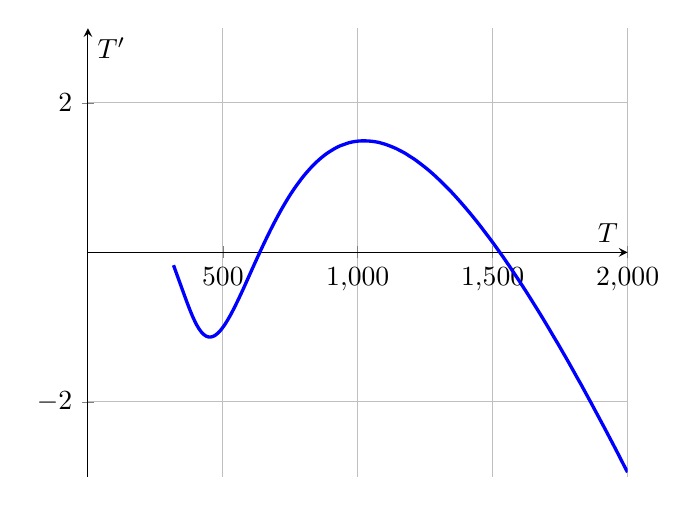
\begin{tikzpicture}
            \begin{axis}[axis lines=center, grid, xmin=0, xmax=2000, ymin=-3, ymax=3,
                domain=300:2000, xlabel={$T$}, ylabel={$T'$}]
                \addplot[smooth, very thick, blue, samples=100] {20*exp(-600/(x-300)) - 0.01*(x-300)};
            \end{axis}
        \end{tikzpicture}
    \end{center}
%     The fixed points are $T_1 = 300^\circ K$, $T_2 \approx 636.8^\circ K$, and $T_3
%     \approx 1526^\circ K$.  $T_1$ is stable from the right, $T_2$ is unstable (above which
%     a combustion occurs), and $T_3$ is stable (stable combustion).
}
% 

\begin{problem}[HIV Problem]
    In a normal, HIV-free body, uninfected T-cells are introduced into the system at a
    constant rate $\lambda$. The T-cells in the system have a finite life span, and hence a
    proportion $\mu$ of the T-cells die. In an HIV infected body, there is a rate $k$ at which
    the T-cells become infected. This rate depends both on the presence of T-cells and
    free HIV-1 particles to infect the T-cells. Putting this together, we get the
    following equation for the healthy T-cells:
    \[ \frac{dT}{dt} = \lambda - \mu T - k TV \]
    where
    \begin{itemize}
        \item $T(t)$ is the number of uninfected and activated T-cells at time $t$
        \item $L(t)$ is the number of latently infected T-cells at time $t$
        \item $I(t)$ is the number of actively infected T-cells at time $t$
        \item $V(t)$ is the number of free HIV-1 particles at time $t$.
    \end{itemize}
    Once a T-cell becomes infected, a proportion $p$ of them will become latently infected,
    while the remainder immediately be actively infected. A latently infected T-cell can
    later become actively infected, and this happens at a rate $\alpha$. Latently infected cells
    die at the same rate $\mu$ as uninfected T-cells. Actively infected T-cells will be
    assumed to die at a different rate $a$. We can now write the equations for the infected
    T-cells:
    \begin{flalign*}
        \frac{dL}{dt} &= kp TV - \mu L - \alpha L \\
        \frac{dI}{dt} &= k(1-p) TV + \alpha L - a I
    \end{flalign*}
    Finally, free HIV-1 particles are manufactured inside actively infected T-cells at a
    rate $c$. The particles die at a rate $\gamma$. The particles are also used in the process of
    infecting healthy T-cells at the rate $k$. This gives us the following equation for
    HIV-1 particles:
    \[ \frac{dV}{dt} = cI - \gamma V - kTV. \]
    Numerically solve system of differential equations and plot the time evolution of all
    four components.  Write a thorough mathematical and biological description of the
    evolution of the system.  The table below gives values for the initial conditions and
    parameters.
    \begin{center}
        \begin{tabular}{|c|l|}
            \hline
            Parameters & Value \\ \hline \hline
            $T(0)$ & 200 T-cells / mm$^3$ \\ \hline
            $L(0)$ & 0 T-cells / mm$^3$ \\ \hline
            $I(0)$ & 0 T-cells / mm$^3$ \\ \hline
            $V(0)$ & $4 \times 10^{-7}$ HIV-1 cells / mm$^3$ \\ \hline
            $\lambda$ & 0.272 / mm$^3$ day \\\hline
            $\mu$ & $1.36 \times 10^{-3}$ / day \\\hline
            $k$ & $2.7 \times 10^{-4}$ mm$^3$/day \\\hline
            $p$ & 0.1 \\\hline
            $\alpha$ & $3.6 \times 10^{-2}$ / day \\\hline
            $a$ & 0.33 / day \\\hline
            $c$ & 100 / day \\\hline
            $\gamma$ & 2 / day \\\hline
        \end{tabular}
    \end{center}
\end{problem}
\hint{
    This is a nonlinear system so use a robust solver.
}



\begin{problem}[Trebuchet Problem]
    A trebuchet catapult throws a cow vertically into the air.  The differential equation
    describing its acceleration is
    \[ \frac{d^2y}{dt^2} = -g - c \frac{dy}{dt} \left| \frac{dy}{dt} \right| \]
    where $g \approx 9.8$ m/s$^2$ and $c \approx 0.02$ m$^{-1}$ for a typical cow.  If the
    cow is launched at an initial upward velocity of 30 m/s, how high will it go, and when
    will it crash back into the ground? Hint: Change this second order differential
    equation into a system of first order differential equations.
\end{problem}
\hint{
    Introduce an auxiliary variable $v = y'$ and write the problem as a system of
    equations.  You will need a robust solver to deal with the nonlinearity in a
    reasonably accurate way (Euler is a bad choice).
}



\begin{problem}[Classical SIR Model]
    When a virus is introduced into a small homogeneously mixed population the people in
    the population can be split into three categories: susceptible to the virus ($S$),
    infected with the virus ($I$), and recovered from the virus ($R$).  Assume the
    following:
    \begin{itemize}
        \item a susceptible person becomes infected at a rate proportional to the product
            of the number of susceptible people and the number of infected people,
        \item the recovery rate is constant,
        \item the recovered people are immune to re-infection,
        \item the virus is not fatal so the total population stays fixed.
    \end{itemize}
    For this problem we will assume that there are $N=1000$ people in the population with
    $I(0) = 1$ person initially infected.
    Your Tasks:
    \begin{enumerate}
        \item[(a)] Write a differential equation for the susceptible population assuming
            that the infection rate is proportional to the product of the sizes of the
            susceptible and infected populations
            \[ \frac{dS}{dt} = \underline{\hspace{1in}}. \]
            (let the proportionality constant be $\alpha$)
        \item[(b)] Write a differential equation for the infected population knowing that
            susceptible people are becoming infected and that infected people are
            recovering at a constant rate
            \[ \frac{dI}{dt} = \underline{\hspace{1in}}. \]
            (let the proportionality constant be $\beta$)
        \item[(c)] Since the total population is fixed in size and only contains the three
            categories we know that $S+I+R = N$ and $\frac{dN}{dt} = 0$.  Hence, the
            differential equations that you wrote in parts (a) and (b) are sufficient for
            modeling the three populations.  Write numerical code that generates a plot of
            the three populations over time.  Fully explore the parameters $\alpha$ and
            $\beta$ and provide several plots that show the different dynamics of the
            problem.
    \end{enumerate}
\end{problem}
\hint{
    \begin{flalign*}
        \frac{dS}{dt} &= -\alpha SI \\
        \frac{dI}{dt} &= \alpha SI - \beta I
    \end{flalign*}
    You can then use the fact that $S+I+R=N$ to get $R = N-S-I$.
}

\begin{problem}[H1N1 Problem]
    The H1N1 virus, also known as the ``bird flu'', is a particularly virulent bug but
    thankfully is also very predicable.  Once a person is infected they are infectious for
    9 days.  Assume that a closed population of $N = 1500$ people (like a small college
    campus) starts with exactly 1 infected person and hence the remainder of the
    population is considered susceptible to the virus.  Furthermore, once a person is
    recovered they have an immunity that typically lasts longer than the outbreak.
    Mathematically we can model an H1N1 outbreak of this kind using 11 compartments:
    susceptible people ($S$), 9 groups of infected people ($I_j$ for $j=1, 2, \cdots, 9$),
    and recovered people ($R$). Write and numerically solve a system of 11 differential equations modeling the
    H1N1 outbreak assuming that susceptible people become infected at a rate proportional
    to the product of the number of susceptible people and the total number of infected
    people. You may assume that the initial infected person is on the first day of their
    infection and determine and unknown parameters using the fact that 1 week after the
    infection starts there are 10 total people infected. 
\end{problem}
\hint{
    The system of equations is
    \begin{flalign*}
        \frac{dS}{dt} &= -\alpha S \left( I_1 + I_2 + I_3 + I_4 + I_5 + I_6 + I_7 + I_8 + I_9
        \right) \\
        \frac{dI_1}{dt} &= \alpha S \left( I_1 + I_2 + I_3 + I_4 + I_5 + I_6 + I_7 + I_8 + I_9
        \right) \\
        \frac{dI_2}{dt} &= I_1 \\
        \frac{dI_3}{dt} &= I_2 \\
        \frac{dI_4}{dt} &= I_3 \\
        \vdots & \\
        \frac{dR}{dt} &= I_9.
    \end{flalign*}
}


\begin{problem}[Pain Management]
    
    When a patient undergoing surgery is asked about their pain the doctors often ask
    patients to rate their pain on a
    subjective 0 to 10 scale with 0 meaning no pain and 10 meaning excruciating pain.
    After surgery the unmitigated pain level in a typical patient will be quite high and
    as such doctors typically treat with narcotics.  
    A mathematical model (inspired by
    \href{https://sinews.siam.org/Details-Page/data-driven-chronic-pain-management-using-hybrid-mathematical-methods}{THIS
    article}
    and \href{https://arxiv.org/pdf/1706.02366.pdf}{THIS paper}) 
    of a patient's subjective pain level as treated pharmaceutically
    by three drugs is given as:
    \begin{flalign*}
        \frac{dP}{dt} &= - \left( k_0 + k_1 D_1 + k_2 D_2 +k_3 D_3\right)P + k_0 u \\
        \frac{dD_1}{dt} &= -k_{D_1} D_1 + \sum_{j=1}^{N_1} \delta (t-\tau_{1,j}) \\ 
        \frac{dD_2}{dt} &= -k_{D_2} D_2 + \sum_{j=1}^{N_2} \delta (t-\tau_{2,j}) \\ 
        \frac{dD_3}{dt} &= -k_{D_3} D_3 + \sum_{j=1}^{N_3} \delta (t-\tau_{3,j})  
    \end{flalign*}
    where
    \begin{itemize}
        \item $P$ is a patient's subjective pain level on a 0 to 10 scale, 
        \item $D_i$ is the amount of the $i^{th}$ drug in the
            patient's bloodstream,
            \begin{itemize}
                \item $D_1$ is a long-acting opioid
                \item $D_2$ is a short-acting opioid
                \item $D_3$ is a non-opioid
            \end{itemize}
        \item $k_0$ is the relaxation rate to baseline pain without drugs, 
        \item $k_i$ is the impact of the $i^{th}$ drug on the relaxation rate, 
        \item $u$ is the patient's baseline (unmitigated) pain, 
        \item $k_{D_i}$ is the elimination rate of the $i^{th}$ drug from the bloodstream, 
        \item $N_i$ is the total number of the $i^{th}$ drug doses taken, and 
        \item $\tau_{i,j}$ are the time times the patient takes the $i^{th}$ drug.
    \end{itemize}
    Implement this model with parameters
    $u=8.01$, $k_0 = \ln(2)/2$, $k_1 = 0.319$, $k_2 = 0.184$, $k_3 = 0.201$, $k_{D_1} =
    \ln(0.5)/(-10)$, $k_{D_2} = \ln(0.5)/(-4)$, and $k_{D_3} = \ln(0.5)/(-4)$.  Take the
    initial pain level to be $P(0) = 3$ with no drugs on board.  Assume that the patient
    begins dosing the long-acting opioid at hour 2 and takes 1 dose periodically every 24 hours.
    Assume that the patient begins dosing the short-acting opioid at hour 0 and takes 1 dose
    periodically every 12 hours.  Finally assume that the patient takes 1 dose of the non-opioid
    drug every 48 hours starts at hour 24.  Of particular interest are how the pain level
    evolves over the first week out of surgery and how the drug concentrations evolve
    over this time.  
    
    \noindent Other questions:
    \begin{itemize}
        \item What does this medication schedule do the patient's pain level?
        \item What happens to the patient's pain level if he/she forgets the non-opioid
            drug?
        \item What happens to the patient's pain level if he/she has a bad reaction to
            opioids and only takes the non-opioid drug?
        \item What happens to the dynamics of the system if the patient's pain starts at
            9/10?
        \item In reality, the unmitigated pain $u$ will decrease in time.  Propose a
            differential equation model for the unmitigated pain that will have a stable
            equilibrium at 3 and has a value of 5 on day 5. Add this fifth differential
            equation to the pain model and examine what happens to the patient's pain
            over the first week. In this model, what happens after the first week if the
            narcotics are ceased?
    \end{itemize}
\end{problem}


\section{Additional ODE Exercises}
\begin{problem}
    Test the Euler, Midpoint, and Runge Kutta methods on the differential
    equation
    \[ y' = \lambda \left( y - \cos(t) \right) - \sin(t) \quad \text{with} \quad y(0) = 1.5. \]
    Find the exact solution by hand using the method of undetermined coefficients and note
    that your exact solution will involve the parameter $\lambda$.  Produce log-log plots
    for the error between your numerical solution and the exact solution for $\lambda =
    -1$, $\lambda = -10$, $\lambda = -10^2$, \ldots, $\lambda = -10^6$.  In other words,
    create 7 plots (one for each $\lambda$) showing how each of the 3 methods performs for
    that value of $\lambda$ at different values for $\Delta t$.
\end{problem}
\hint{
    Let the maximum time be small and take a large number of time steps.
}

\begin{problem}
    Write code to solve the boundary valued differential equation
    \[ y'' = \cos(t) y' + \sin(t) y \quad \text{with} \quad y(0) = 0 \quad \text{and}
        \quad y(1) = 1. \]
\end{problem}
\hint{
    Introduce an auxiliary variable $v = y'$ and write the problem as a system of
    equations.
}

